\section{Introduction}
\label{sect:intro}

\noindent
Probabilistic inference in many real-world problems requires graphical
models with deterministic algebraic constraints between random
variables.
%Probabilistic inference in many real-world problems often requires
%graphical models with (non)linear constraints between random
%variables.  Such constraints appear in case instead of direct
%observation of random variables, deterministic functions of them are
%observed.
Consider the following running example from physics and the
associated graphical model of Figure~\ref{fig:collision.bn}:

\noindent{\bf Collision model. }
\emph{
Masses $M_1$ and $M_2$ with velocities $V_1$ and $V_2$ collide to form a single mass $(M_1 + M_2)$ with total momentum 
$P_\text{tot} = M_1 V_1 + M_2 V_2$ (assuming that there is no dissipation).
The prior density of masses and velocities are:\footnote{
$\mathcal{U}(a, \, b)$ denotes a uniform density with support $[a,b]$.}
\begin{align}
&\pr(M_1) = \mathcal{U}(0.1, \, 2.1), \quad 
&&\pr(M_2) \!=\! \mathcal{U}(0.1, \, 2.1) \label{sym:u12}\\
&\pr(V_1) = \mathcal{U}(-2, \, 2), \quad
&&\pr(V_2 \, | \, V_1) = \mathcal{U}(-2, \, V_1) \label{sym:u34}
%\label{e:collision}
\end{align}
The total momentum is observed to be $3.0$.
\begin{align}\label{f:p_tot}
P_{tot} = M_1 V_1 + M_2 V_2 = 3.0
\end{align}
}%end emph

\begin{figure}
\center
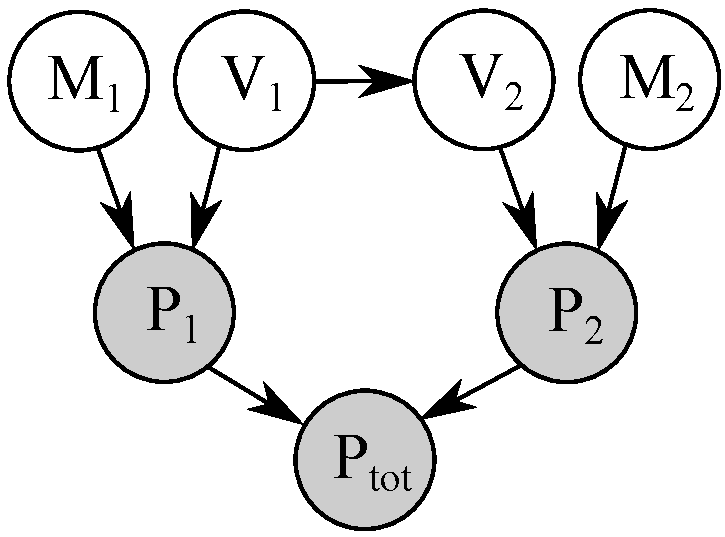
\includegraphics[width=0.15\textwidth]{Figs/little-momentum1.pdf} 
\vspace{-2mm}
\caption{\footnotesize Bayesian network of the \emph{collision model}. Shaded circles correspond random variables that are functions of other variables.}
\label{fig:collision.bn}
\vspace{-5mm}
\end{figure}



 
%In applications of probabilistic inference, instead of direct observation of random variables (e.g., $X$ and $Y$), functions of them may be observed (e.g., $X\cdot Y = c$).

In such problems, the posterior densities only have support on (non)linear sub-manifolds of the parameter space (e.g.\ a hyperplane in the collision model). 
Efficient inference on such models is extremely challenging \cite{pennec2006intrinsic}. 

To evade the complications, state-of-the-art MCMC based probabilistic inference tools suggest adding noise to the observation (hard to soft constraint conversion) \cite{wood2014new}. 
Nonetheless, this strategy does not help much: If the added noise is large then the approximation bounds can be arbitrarily large and if it is small, the sampling mixing rate can be arbitrarily slow \cite{li2013dynamic,chin1987bayesian}. 
 
The other potential solution is to reduce the dimensionality of the posterior distribution via Jacobian-based random variable transformations. Measure theoretic subtleties aside, such transformations are only applicable when the observed function is invertible with respect to at least one random variable. Using the properties of the Dirac delta, our first contribution is to propose a dimension reduction method that is more general in the sense that the observed function is not required to be invertible but should be solvable with one or several distinct roots. Up to our knowledge, this is the first time that Dirac delta is used in this context.
Nonetheless, dimension reduction (either carried out via Jacobian-based or Dirac delta-based mechanism) does not completely eliminate the problem since as it will be shown shortly, the produced low dimensional distributions are highly piecewise and multimodal. 

Exact inference on such models is almost never possible and the convergence rate of the approximate alternatives can be extremely low.
For instance,
the leapfrog mechanism by which Hamiltonian Monte Carlo (HMC) simulates the Hamiltonian dynamics relies on the assumption of smoothness \cite{neal2011mcmc}.
This assumption does not hold 
 in the adjacency of discontinuities (borders of pieces) leading to low proposal acceptance rates and poor performance. 
Slice sampling suffers from the multimodal nature of the distributions that are in the focus of  the present work. Similarly, near the borders of partitions, the acceptance rate of Metropolis-Hastings(MH) is typically low since in such areas the difference (e.g.\ KL-divergence) between MH’s \emph{proposal distribution} and the suddenly varying target distribution is often significant.
The exception is Gibbs sampling. The latter method can be regarded as a particular variation of MH where the proposals are directly chosen from the target distribution and therefore follow the target distribution changes and multimodalities.
Nonetheless, Gibbs samplers can be quite slow since the per sample computation conditionals that Gibbs relies on are costly and in general cannot be performed in closed form.    

As such, in the second part of the paper we address the problem of sampling from highly piecewise distributions. %by proposing a variation of Gibbs sampling that saves a tremendous amount of redundan 
We firstly introduce a reach class of \emph{piecewise fractional functions} as a building block for piecewise graphical models.% with (non)linear observed constraints.  
We show that this class is closed under the operations required for Dirac delta-based dimension reduction.
This class is rich enough to approximate arbitrary density functions up to arbitrary precision. 
We further show that the form of resulting collapsed model always permits one closed-form integral -- sufficient to analytically derive conditionals for Gibbs sampling prior to the sampling process which saves a tremendous amount of computations.
We evaluate this fully-automated sampler for models motivated by physics and engineering and show it converges at least an order of magnitude faster than existing MCMC samplers, thus enabling probabilistic reasoning in a variety of applications that, to date, have remained beyond the tractability and accuracy purview of existing inference methods.  

%We firstly introduce a highly expressive family of piecewise models (called PPF* for \emph{polynomial piecewise fractionals}) that consists of real-space piecewise distributions where the partitioning hyperplanes are made of polynomials where the degree of each variable is at most 2 and the function value in each partition has a fractional form where the denominator is factorized into terms where the degree of each variable is at most 2. We show that univariate integrals (w.r.t.\ any variable) of such piecewise functions can always be computed analytically. Symbolic Gibbs works on such models. Its basic idea is to  construct a mapping from variables to their associated univariate analytic CDFs that are computed prior to the sampling process. By this trick, the actual CDF computations per sample is reduced the instantiation of the symbolic CDFs that are associated with each variable. This saves a tremendous amount of redundant computations and leads to a sampler that is at least an order of magnitude faster than the baseline.

%Note that the reference family of models, PPF*, is rich enough to approximate arbitrary distributions up to arbitrary precision. It should also be pointed out that handling observed deterministic constraints is only one application of symbolic Gibbs since the latter algorithm is applicable to any piecewise or non-piecewise PPF* model.  Nonetheless, due to the importance of inference in presence of determinism and the fact that this problem is not tackled in a systematic and automated way so far, we only focus on this specific throughout.


%...............

%Probabilistic inference in many real-world problems often requires graphical models with nonlinear deterministic constraints between random variables (e.g., laws of physics) and piecewise distributions (e.g., priors enforcing bounded parameter values).  To date, exact inference in graphical models with piecewise factors has been restricted to piecewise polynomial/exponential factors with hyperrectangular, hyper-rhombus or linear partitioning constraints~\cite{shenoy2011inference,shenoy2012two,Sanner:12} and has altogether ignored the complications of (nonlinear) determinism. Observed determinism can appear in applications such as failure detection \cite{huseby2004system} where random variables $X_1, \ldots X_k$ are not directly observable but a function $f(X_1, \ldots, X_k)$ of them may be observed (indirect measurement). Some families of distributions such as \emph{conditional linear Gaussians} (CLGs) \cite{lauritzen2001stable} are closed under linear transformations and consequently allow \emph{linear determinism}.
% TODO: The following makes no sense and is not written in a precise
%       academic style with clear conclusions.  It also breaks the
%       flow of discussion from linear to nonlinear.  I am dropping
%       the explanation and simply adding a \nocite to ensure the ref
%       shows up in the bib.  -Scott \nocite{li2013dynamic}
%In \cite{li2013dynamic} the restriction is imposed on the network topology rather than the densities. They can only handle the observed summation of variables on a very simple Bayesian network. The generalization of this technique does not seem straight-forward (if possible).

%Handling nonlinear determinism is much more difficult. Methods based on Hamiltonian Monte Carlo are used for sampling under particular constraints \cite{hartmann2008ergodic} but they perform poorly in piecewise models (due to poor approximation of Hamiltonian dynamism in discontinuities)~\cite{neal2011mcmc}.  \cite{cobb2005nonlinear} approximate nonlinear determinism with piecewise linear constraints by dividing the space into hypercubes. This method cannot be used beyond three dimensions since the number of partitions required to preserve approximation accuracy is exponential in dimensionality. The solution often suggested by probabilistic programming languages is to approximate the observed determinism by adding noise to the observation (i.e., a hard to soft constraint relaxation). However, in practice if the added noise is large, the approximation bounds may become arbitrarily large and if the noise is small, the mixing rate may become extremely slow (near-deterministic problem) \cite{chin1987bayesian}.  In short, inference conditioning on nonlineardeterminism is still an open problem \cite{li2013dynamic}. 

%In this paper, we introduce a rich class of \emph{polynomial piecewise  fractional functions} (PPFs) as a building block for piecewise graphical models with nonlinear deterministic constraints.  We show that deterministic constraints in these models can always be eliminated through collapsing.  We further show that the form of the collapsed model always permits one \emph{symbolic} integral --- sufficient to \emph{automatically} derive conditionals for Gibbssampling.  We evaluate this fully automated \emph{Symbolic Gibbs} sampler for nonlinear piecewise graphical models on examples motivated by physics and engineering and show it converges an order of magnitude faster than existing Monte Carlo samplers, thus enabling probabilistic reasoning in a variety of applications that, to date, have remained beyond the tractability and accuracy purview of existing inference methods.

% Somewhat incoherent!  -Scott
\begin{comment}
As we will show, a large subset of this family 
(1) remain closed under operations such as algebraic fractional substitutions.
(2) have closed-form univariate integrals.
The former property makes PPFs an important tool 
in fully-automated reasoning conditioned on (non)linear deterministic constraints between model random variables (see Section\ref{sect:determinism})
and the latter property makes them an appropriate application of \emph{exact} Gibbs sampling. 
In the sense that the univariate CDF computations required in each step of Gibbs sampling can be computed in closed-form and prior to the sampling process. 
 In this way, we create a \emph{symbolic
  Gibbs} algorithm that saves a significant amount of computation by avoiding
per-sample computations, and shows dramatically improved performance
compared to existing samplers on complex models motivated by physics
and engineering. 
\end{comment}
